\documentclass[a4paper]{tufte-handout}

\title{The digimorse Communications Protocol}
\author{ Matt Gumbley, M{\O}CUV}

%\date % without \date command, current date is supplied

%\geometry{showframe} % display margins for debugging page layout


% The tufte-latex package is great for pdflatex, but TeXPad uses xelatex, which fouls up the header, and doesn't build unless the following section is added. The header doesn't use a smallcaps font, and I had to change the main text and math font to make it look a bit better...

% Thanks to https://tex.stackexchange.com/questions/200722/xetex-seems-to-break-headers-in-tufte-handout
\usepackage{fontspec}
\usepackage{ifxetex}


\ifxetex
  \newcommand{\textls}[2][5]{%
    \begingroup\addfontfeatures{LetterSpace=#1}#2\endgroup
  }
  \renewcommand{\allcapsspacing}[1]{\textls[15]{#1}}
  \renewcommand{\smallcapsspacing}[1]{\textls[10]{#1}}
  \renewcommand{\allcaps}[1]{\textls[15]{\MakeTextUppercase{#1}}}
  \renewcommand{\smallcaps}[1]{\smallcapsspacing{\scshape\MakeTextLowercase{#1}}}
  \renewcommand{\textsc}[1]{\smallcapsspacing{\textsmallcaps{#1}}}
\fi

\setmainfont[Renderer=Basic, Numbers=OldStyle, Scale = 1.0]{Palatino}

% Get the small caps right. Too much fiddling going on when using xelatex and tufte-latex.
% The title and author aren't as nice as with pdflatex, but at least it builds.
\setmainfont{texgyrepagella}[
 Path = /opt/local/share/texmf-texlive/fonts/opentype/public/tex-gyre/ ,
 UprightFont = *-regular ,
 BoldFont = *-bold ,
 SmallCapsFeatures={Letters=SmallCaps},
]

\setsansfont[Renderer=Basic, Scale=0.90]{Helvetica}

\usepackage{graphicx} % allow embedded images
\setkeys{Gin}{width=\linewidth,totalheight=\textheight,keepaspectratio}
\graphicspath{{graphics/}} % set of paths to search for images
\usepackage{amsmath}  % extended mathematics
\usepackage{booktabs} % book-quality tables
\usepackage{units}    % non-stacked fractions and better unit spacing
\usepackage{multicol} % multiple column layout facilities
\usepackage{lipsum}   % filler text
\usepackage{fancyvrb} % extended verbatim environments
\usepackage{hyperref} % URLs
\usepackage{xcolor}   % For coloured text
\usepackage{soul}     % For highlighted text
\fvset{fontsize=\normalsize}% default font size for fancy-verbatim environments

% Standardize command font styles and environments
\newcommand{\doccmd}[1]{\texttt{\textbackslash#1}}% command name -- adds backslash automatically
\newcommand{\docopt}[1]{\ensuremath{\langle}\textrm{\textit{#1}}\ensuremath{\rangle}}% optional command argument
\newcommand{\docarg}[1]{\textrm{\textit{#1}}}% (required) command argument
\newcommand{\docenv}[1]{\textsf{#1}}% environment name
\newcommand{\docpkg}[1]{\texttt{#1}}% package name
\newcommand{\doccls}[1]{\texttt{#1}}% document class name
\newcommand{\docclsopt}[1]{\texttt{#1}}% document class option name
\newenvironment{docspec}{\begin{quote}\noindent}{\end{quote}}% command specification environment



\begin{document}

    \maketitle % this prints the handout title, author, and date

    \begin{abstract}
        \noindent
        This document introduces an experimental alternative to amateur radio's traditional way of transmitting Morse code.
        It describes the rationale for, and the design of the digimorse communications protocol.
        The design is explained in the context of general digital communications systems, with
        discussions of the choices made at all stages of its implementation in the transceiver software.
    \end{abstract}

    \newthought{The digimorse communications protocol exists} to bring together two aspects of amateur radio that I
    particularly
    enjoy, to see if the benefits of one aspect might improve my enjoyment of the other.
    Namely, to see if digital encoding and error correction\footnote{Such as found in the WSJT-X weak-signal mode
    software by Joe Taylor K1JT et al.} might be used to provide a significant coding gain and a removal of noise
    from Morse Code - our historic mode of communication.

    Other features of modern digital amateur radio that I aim to bring to Morse operation with digimorse include:
    \begin{itemize}
        \setlength\itemsep{-0.5em}
        \item a waterfall display
        \item active station information
        \item meaningful signal reports
    \end{itemize}

    Waterfall displays are now standard features on modern SDR\footnote{Software Defined Radio} transceivers such as
    the Yaesu FTDX10, and in software such as WSJT-X\cite{FT4FT8}.
    They graphically show the presence of any signals - and information about their senders - across the receiver's
    audio bandwidth.
    The decode window of WSJT-X shows the content of the decoded messages that have been received in recent
    receive cycles.
    With this display it is easy to see who is currently active on the band, how strong their signals are, and their
    country/locator square.
    This gives an excellent overview of propagation conditions and band activity.
    Signal reports are automatically derived from the incoming signal strength, and are therefore meaningful – rather
    than the typical ‘you are 5 by 9… what was your name and callsign again?’.

    With digimorse, since the Morse code you send is encoded and decoded digitally, if the receiving station
    achieves a successful decode, the code will be played back exactly as it was sent, with no noise.

    In amateur radio, Morse code is traditionally transmitted using a pure sinusoidal radio wave, oscillating at a
    fixed frequency. This gives rise to the name and acronym it is more commonly known as: Continuous Wave, or CW.
    This method of transmitting Morse originated around 1913, with the invention of the \emph{vacuum tube electronic
    oscillator} by Edwin Armstrong and Alexander Meissner\footnote{See Wikipedia, 'Continuous wave'}. Prior to this,
    Morse was transmitted using primitive \emph{spark gap} transmitters, which created much electromagnetic
    interference, and had wide bandwidth. They were outlawed in 1934. The bandwidth of a CW signal is very low,
    compared to the systems it replaced\cite{Amos}.

	\pagebreak
    Perhaps surprisingly, CW, as a method of transmitting Morse code
    using radio, has not changed significantly since then. In the intervening years, great improvements to receiver
    technology have been made: receiver sensitivity and selectivity have improved; filtering and digital signal
    processing techniques have been applied to try to reduce or remove the noise that plagues reception.

    However, despite these advances, noise and fading effects introduced by ionospheric reflection still impact our
    ability to receive and decode Morse, as received using CW signals.

    As an analogy, digimorse intends to do to Morse code what compact discs did for vinyl recordings. It's an upgrade
    for CW.

    This paper introduces digimorse in the context of modern digital communications protocols for the radio amateur.

    \pagebreak
    \tableofcontents
    \pagebreak

\section{Overview of the digimorse transceiver}
    \newthought{A view of the functions of the digimorse transceiver}, to be explored more fully in later sections.

\subsection{Transmission}

    The digimorse software uses real, hand-sent Morse Code - not typed, computer-generated 'perfect' Morse - but keyed
    on a straight key, or paddle\footnote{Only straight keys are currently supported.}.
    The key or paddle is attached to the computer via an Arduino-based USB interface which samples your keying,
    sending a stream of millisecond-precise key up/down durations to the computer.
    In addition to sampled keying information, several other ‘metadata’ items are included in the outgoing stream of
    frames – callsign, location, keying speed and power.
    This stream is then compressed, protected by a CRC\footnote{Cyclic Redundancy Check.} error-detection code, then
    enhanced with an LDPC\footnote{Low-Density Parity-Check} error-correction code\cite{Gallager1962} - similar to
    that used in FT4/FT8.
    These measures mitigate the effects of noise and other interference during receive, thereby improving the ability
    of the software to correctly decode extremely weak signals.
    These blocks of data are then prefixed with a Costas array\cite{Hasselbeck2019}, to allow the receiver to 
    precisely filter the frame stream from the rest of the received audio.
    The complete stream is then modulated into a narrow bandwidth of tones, taking care to minimise splatter.
    Many such transmissions can occur simultaneously within a transceiver’s 3kHz SSB bandwidth.
    The resultant audio is then transmitted.

\subsection{Reception}

    The receiver detects all narrow-bandwidth digimorse signals across its 3kHz incoming audio bandwidth by searching
    for their initial Costas arrays.
    After demodulation, error detection and correction is applied, and if the stream is valid, the detected metadata
    frames are displayed above each stream of keying information so that you can easily see who is
    transmitting, from where, how strong their signals are, and how fast they are keying.
    Given this scrolling display of decoded streams, you may select individual signals, or apply a bandpass filter
    across part of the receive bandwidth.
    The result is that the single selected signal - or multiple filtered signals - are then decoded, and
    reconstituted into high-quality Morse code, with no noise.
    Each stream is located at some audio offset from the start of the 3kHz receiver bandwidth, and this offset is used
    as the tone for each signal.
    The inclusion of LDPC error correction information means that even if your RF signal is very weak at the
    receiver, with high levels of noise present, then some or all of your transmission should be decodable, giving a
    considerable coding gain over CW~\cite{Punch2013}.

\pagebreak
\section{Digital Communications Systems}
\newthought{The overview presented above will now be expanded upon} by reviewing a generic
    digital communications system, and then explaining how each of its building
    blocks is implemented in digimorse.

    Claude Shannon presented a high-level variant of the following diagram in his seminal paper "A Mathematical
    Theory of Communication"\cite{Shannon1948}. The diagram shown below is a modern enhancement for digital
    communication systems.

    All of the modern digital communication systems you might use adhere to this same basic structure.

    \begin{figure*}[h]
        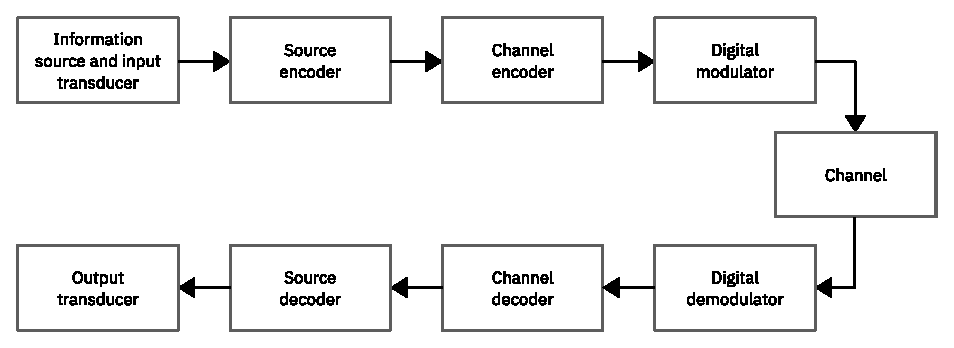
\includegraphics[width=\linewidth]{images/digital-communication-system}
        \caption{Basic elements of a digital communications system}
        \label{fig:digcomms}
    \end{figure*}

    % EXPLAIN WHAT'S GOING ON HERE AT THE HIGH LEVEL

    The diagram starts at the top-left, and illustrates the path taken by some information (a \emph{message}) from
    its source, to its eventual destination.
    The source could be analogue or digital, and is encoded into some digital form, such that it can be expressed in
    as few binary digits as possible.
    The output of the source encoder should exhibit as little \emph{redundancy} as possible; it should be as
    \emph{compressed} as possible.

    The resulting \emph{information sequence} is then fed to the channel encoder, which is tasked with preparing it
    for its journey through the channel.
    This is achieved by adding some redundancy back into the information, but in a structured manner, such that it
    can be used by the receiver to overcome the effects of noise and interference presented by the transmission over
    the channel.
    The reliability of decoding during reception is increased by this added redundancy.

    The binary output of the channel encoder must be converted into a form suitable for transmission over the
    channel: this is the function of the digital modulator, which typically maps binary data into electrical signal
    waveforms.

    The channel is the physical medium through which the signal is sent from transmitter to receiver. In amateur
    radio, this is the atmosphere, either a transmission via ground wave or sky wave. In either case, the signal is
    subject to interference, and is corrupted randomly by noise generated by other electronic devices, atmospheric
    noise (e.g. lightning discharges), human-generated noise such as car ignition noise or other switching. It can
    also be subject to various types of fading, multipath reflection, doppler effects, etc.


	% TODO discuss digital demodulator
	\hl{discuss digital demodulator}
	% TODO discuss channel decoder
	\hl{discuss channel decoder}
	% TODO discuss source decoder
	\hl{discuss source decoder}
	% TODO discuss output transducer
	\hl{discuss output transducer}
	

    Starting with Morse code, I will now discuss each of these building blocks in turn, and their design and implementation in digimorse.


\section{digimorse as a Digital Communications System}
    \newthought{Before taking several deep dives} into the building blocks, let's zoom out a little further, and look at the whole of digimorse - as there are additional parts that don't appear in the previous description of generic digital communications systems. 


%TODO include full block diagram
	\hl{full block diagram goes here}
	    
    % FRAME THE PROBLEM AND PROVIDE MOTIVATION AND BACKGROUND. SAY WHAT THE PROBLEM IS, STATE THE OUTPUT AND KEY IDEA
    % BEFORE DISCUSSING STEPS.

\section{Information Source and Input Transducer}

Morse key and Arduino, keying protocol, USB Serial, protocol decoder, keying event stream.
how the protocol decoder is wired to other block diagram elements.
\hl{more, obvs}

\section{Source Encoder}
Given a stream of keying information from the input layer, this must be encoded into a compressed form to remove redundancy, ensuring that the minimum number of bits are used (since the transmission of bits takes time; fewer bits are better).

The output of the source encoder is a fixed-length binary block of \hl{UNDECIDED} bits. Keying and other metadata frames are appended to this block until:
\begin{itemize}
    \setlength\itemsep{-0.5em}
	\item It is full.
	\item Until the frame being appended will not fit at the end, causing the block to be filled with a padding frame. The frame will then be stored at the start of the next block.
\end{itemize}
The block is then sent on to the next major component in the transceiver, the channel encoder.
The need for a fixed-length block is due to the channel encoder, whose error-correction algorithm requires it.

The full set of frame types that may be incorporated in the block is given in the following table on page \pageref{table:frame-types}.

    \marginnote{The XXX|N notation means that the XXX value is encoded as an N-bit unsigned binary number.}
    \begin{table}[h]

        \fontfamily{ppl}\selectfont
        \begin{tabular}{lll}
            \toprule
            4-Bit Frame Id & Description & Encoding \\
            \midrule
            0000 & Padding to end of block &  \\
            0001 & WPM/Polarity & WPM|6; Polarity|1 \\ 
            0010 & MD Callsign & Callsign|28 \\
            0011 & MD Callsign hash & Hash|22 \\
            0100 & MD 4-Character Locator & C15 \\
            0101 & MD Power & xxx \\
            0110 & Keying (Perfect dit) & \\
            0111 & Keying (Perfect dah) & \\
            1000 & Keying (Perfect wordgap) & \\
            1001 & Keying (End) & \\
            1010 & Keying (Delta dit) & See page \pageref{section:delta-encoding} \\
            1011 & Keying (Delta dah) & \\
            1100 & Keying (Delta wordgap) & \\
            1101 & \emph{unused} & \\
            1110 & \emph{unused} & \\
            1111 & Extension & To be considered later... \\
		\end{tabular}
		\caption{Frame types and their data, encoded into blocks by the source encoder.}
		\label{table:frame-types}
	\end{table}

When a frame has been added to a block, if there are fewer than four bits remaining, they are assumed to be padding, so the frame is emitted, and a new frame started.

In addition to the keying duration information, the source encoder must also encode the current speed in WPM, and the polarity of the key at the start of the frame. This ensures that in the event of a receiver being unable to correctly decode a frame, it will be able to 'pick up' the stream when it next has a successful decode. The WPM of the frame is sent in each frame\footnote{In each frame that contains keying information. Most would.} to ensure that the compressed keying duration data is correctly interpreted: it is expressed as a delta against the ideal timings - see page \pageref{section:delta-encoding}.

Callsign and locator encoding are performed using the same mechanism as in JT65.\cite{ClarkKarn1996}

The source encoder contains a rudimentary 'CQ detector' that detects when CQ has been sent at the start of a transmission. When this finds a CQ, it forces the source encoder to start embedding metadata frames. The current block will contain the Callsign frame; the next block will contain the 4-Character Locator frame; the next block will contain the Power frame.

Also if a Callsign frame has not been embedded in a block for 15 minutes, one will be included in the current block.\footnote{This timed callsign does not cause the next block to contain the 4-Character Locator as described in the previous paragraph.}

This mechanism ensures that all metadata is sent close to the start of a CQ, spread across subsequent blocks\footnote{So as to prevent 'starvation' of keying information in a single block.} so that receiving users decode the metadata of all stations calling CQ. It also ensures compliance with regulations that require a station identify itself frequently. 

If a block does not contain a Callsign, then it will contain a Callsign Hash, which is a much smaller length frame than a Callsign. Either of these can be used in the receiver to enable the decoding and playback of a single station's transmission. By selecting the station's metadata, it is possible to filter out all other keying streams. This could be done by choosing a narrow bandwidth filtering range, but that would not reject another station whose offset is very close to the DX station. By including the Callsign or Callsign Hash in each block, the stream can be identified precisely.\footnote{Hash collisions notwithstanding!}

A block will only contain one metadata frame (as indicated by MD in the table above). 


If the operator has perfect rhythm and timing, and their dits, dahs and wordgaps are precisely the correct duration for the current WPM setting, then the 'Perfect dit/dah/wordgap' frames will be used, as these require no further data than their 4-bit frame id.

This would be the case if digimorse eventually accommodates a machine-generated stream of Morse, perhaps by entering text on-screen, or by the use of macro buttons. This could also happen when the USB interface is enhanced to incorporate a keyer.\marginnote{I'm not in favour of making digimorse highly automated - the rationale of the project is to enhance the human enjoyment of Morse, not replace human operation by computer operation. You could use PSK31, RTTY, FT8 etc. for that.}

For the rest of us mortal operators with our shaky fists and dodgy timing, digimorse will try to record and reproduce our variations as precisely as it can, given its millisecond resolution.

The digimorse transceiver accommodates keying speeds of 5 to 60 words per minute. There are three major \emph{timing elements} in Morse: the \emph{dit}, the \emph{dah}   and the \emph{wordgap}.\marginnote{A clear description of the elements and how they are used to form words is given by Michael Maynard K4ICY, illustrating the 'standard word' \textsc{PARIS}, used for calculating keying speed in words-per-minute.\cite{Maynard}}

A table showing the durations in milliseconds for these three elements, for all speeds in this range is given in the appendix on page~\pageref{tab:morsetab}. The longest element that could be transmitted is the 5WPM wordgap at 1680ms; the shortest is the 60WPM dit at 20ms. An operator could pause for longer than 1680ms of course, until the keyer times out and sends an End signal which terminates transmission.\marginnote{This timeout can be configured in the keyer up to 3000ms i.e. three seconds.}

How should this range of timings be encoded in the most compact form?


\subsection{Naïve encoding}

The longest duration of 1680ms could be encoded by $\log_2\left(1680\right) = 10.714$, and so could be expressed as a binary field of 11 bits, as could any value up to 2047. This \emph{naïve} approach to encoding could work\marginnote{Do The Simplest Thing That Could Possibly Work}, but would be inefficient, as will be shown next.


\subsection{Delta encoding based on code speed}
\label{section:delta-encoding}

I took an example of a typical Morse QSO\cite{Summers} and keyed it into digimorse using the \textsc{KeyerDiag} option, which records your keying into a .CSV file containing MARK/SPACE duration data, and plays a sidetone as you operate.
The resulting data is shown as a histogram in Figure \ref{fig:sampleqso} on page \pageref{fig:sampleqso}. Several aspects of this are worth pointing out:
\begin{itemize}
    \setlength\itemsep{-0.5em}
    \item The modal value in the data is 72ms, so taking this as the duration of a dit, this suggests (from Appendix A) a speed between 16 and 17 WPM - say 16. This gives a dah of 225ms and a wordgap of 525ms. These ideal durations are shown with the three vertical bars.

	\item dit is far more common than dah or wordgap.
	\item There is no large spike for dah - the peak nearby is at a longer duration than the ideal, so my dah is slow. There is no spike at all for wordgap - just a smattering of points - indicative of the relative frequency of word gaps in the text.
	\item The points around these ideal timings are not as pronounced as they are for dit - suggesting I have a wide variance in my keying of the longer elements, but I'm more accurate with dit.

\end{itemize}  

To reduce the number of bits required to encode keying, determine whether the duration is closest to dit, dah or wordgap for the current WPM setting, then take the difference between this ideal duration and the value under consideration.

%TODO encode the distance from the dit/dah/wordgap based on the selected speed	

    \begin{figure*}[h]
        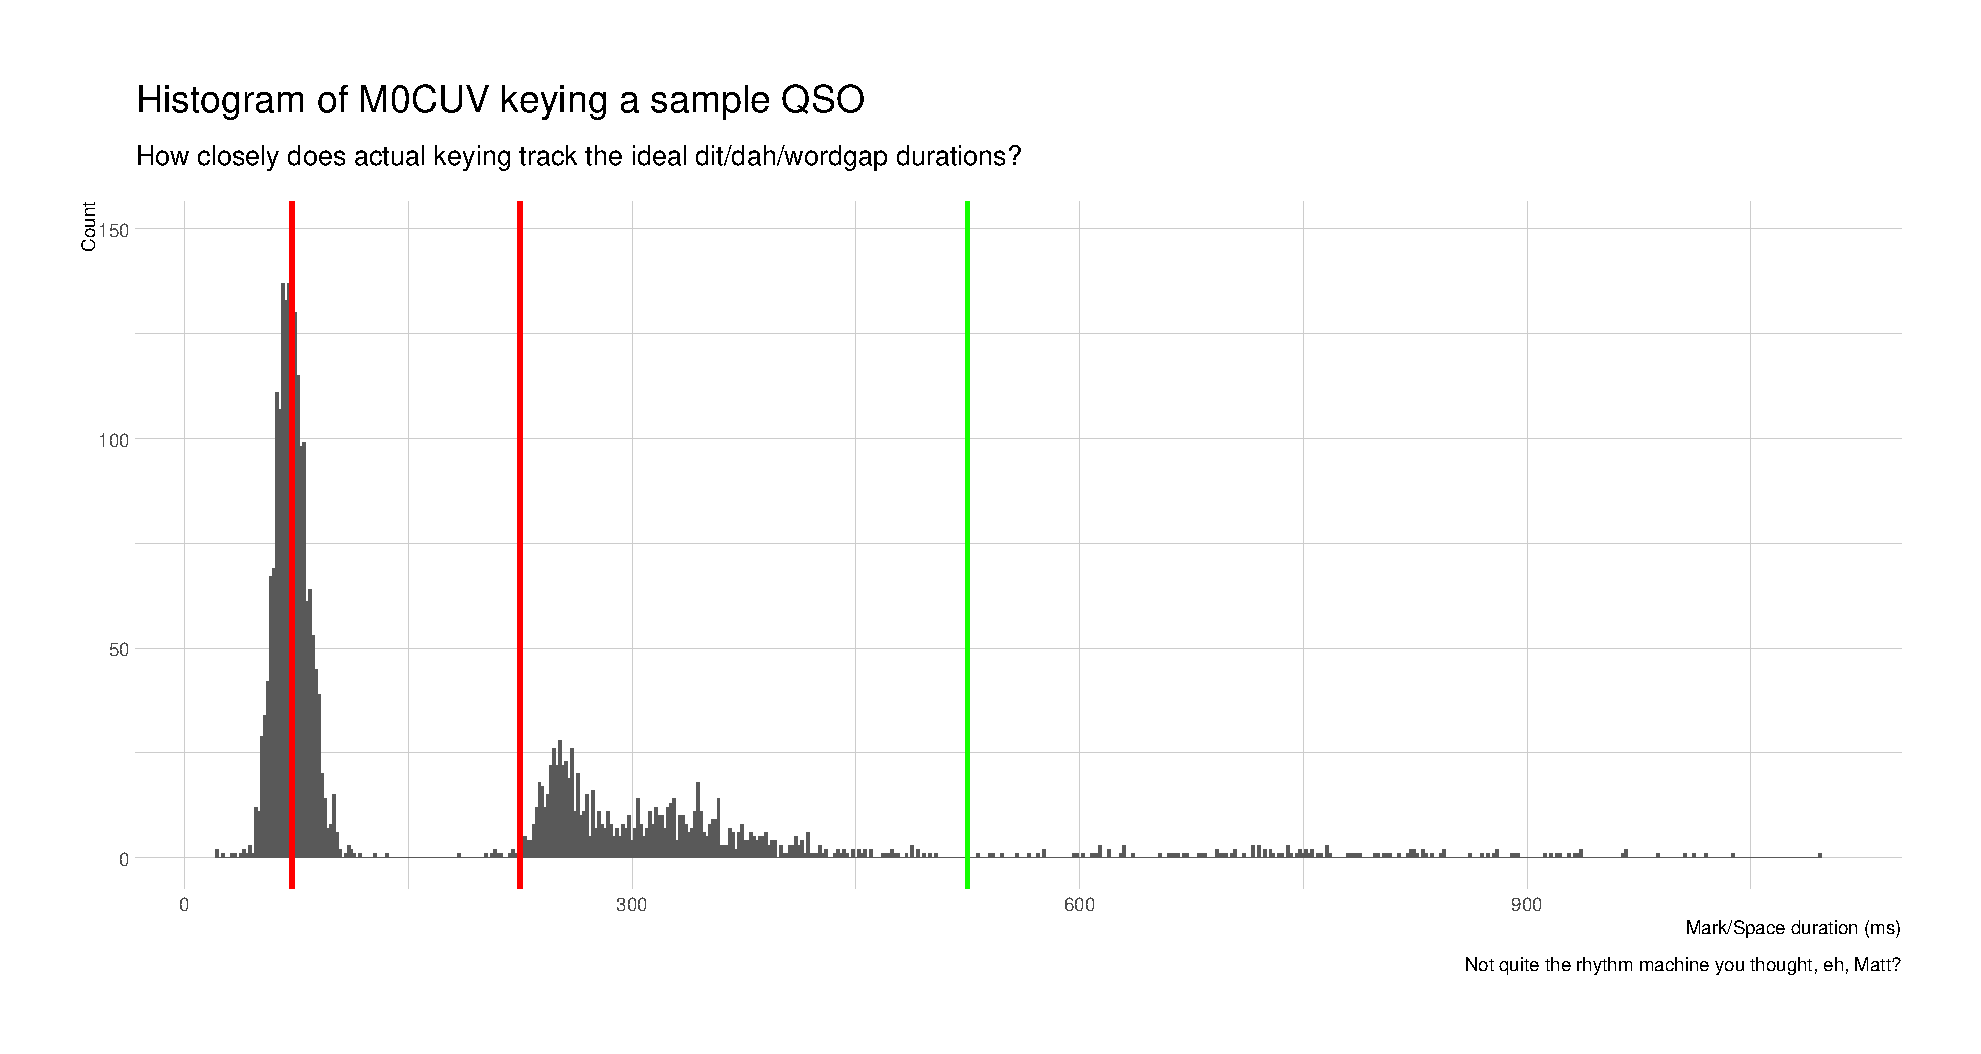
\includegraphics[width=\linewidth]{sample-qso-m0cuv}
        \caption{Keying of a sample QSO}
        \label{fig:sampleqso}
    \end{figure*}


\section{Channel Encoder}
Adding LDPC and CRC \& Costas Array. End of transmission marker (another Costas array?).

\section{Digital Modulator}
8-GFSK modulation? Bandwidth vs transmission speed.

\section{Channel}
Typically HF or VHF, SSB 3kHz.

\section{Digital Demodulator}
Detecting Costas array, training narrow bandwidth filter on incoming signals. 

\section{Channel Decoder}
Apply LDPC and CRC to recover frame. Output is a binary frame.
Second pass to recover signals on top of each other?

\section{Source Decoder}
Given a binary frame that's correct, process its metadata.

\section{Output transducer}
If the decoded frame is within the current audio filter bandwidth, enqueue the Morse keying at the appropriate frequency.

\section{Miscellaneous topics}
The CQ detector. Transmit/receive switching.

\pagebreak
\section{Project Website}

The website for the digimorse protocol and transceiver software is located at
\url{https://devzendo.github.io/digimorse}. On the website, you'll find
links to our \smallcaps{git} repository, mailing lists, bug tracker, and documentation.

\pagebreak
\appendix
\section*{Appendices}
\addcontentsline{toc}{section}{Appendices}
\renewcommand{\thesubsection}{\Alph{subsection}}

\subsection{Morse Code Speeds}

    \begin{table}[!h]
        \footnotesize
        \centering
        \fontfamily{ppl}\selectfont
        \begin{tabular}{llll}
            \toprule
            WPM & ms/dit & ms/dah & ms/wordgap \\
            \midrule
            5 & 240 & 720 & 1680 \\
            6 & 200 & 600 & 1400 \\
            7 & 171.4285714 & 514.2857143 & 1200 \\
            8 & 150 & 450 & 1050 \\
            9 & 133.3333333 & 400 & 933.3333333 \\
            10 & 120 & 360 & 840 \\
            11 & 109.0909091 & 327.2727273 & 763.6363636 \\
            12 & 100 & 300 & 700 \\
            13 & 92.30769231 & 276.9230769 & 646.1538462 \\
            14 & 85.71428571 & 257.1428571 & 600 \\
            15 & 80 & 240 & 560 \\
            16 & 75 & 225 & 525 \\
            17 & 70.58823529 & 211.7647059 & 494.1176471 \\
            18 & 66.66666667 & 200 & 466.6666667 \\
            19 & 63.15789474 & 189.4736842 & 442.1052632 \\
            20 & 60 & 180 & 420 \\
            21 & 57.14285714 & 171.4285714 & 400 \\
            22 & 54.54545455 & 163.6363636 & 381.8181818 \\
            23 & 52.17391304 & 156.5217391 & 365.2173913 \\
            24 & 50 & 150 & 350 \\
            25 & 48 & 144 & 336 \\
            26 & 46.15384615 & 138.4615385 & 323.0769231 \\
            27 & 44.44444444 & 133.3333333 & 311.1111111 \\
            28 & 42.85714286 & 128.5714286 & 300 \\
            29 & 41.37931034 & 124.137931 & 289.6551724 \\
            30 & 40 & 120 & 280 \\
            31 & 38.70967742 & 116.1290323 & 270.9677419 \\
            32 & 37.5 & 112.5 & 262.5 \\
            33 & 36.36363636 & 109.0909091 & 254.5454545 \\
            34 & 35.29411765 & 105.8823529 & 247.0588235 \\
            35 & 34.28571429 & 102.8571429 & 240 \\
            36 & 33.33333333 & 100 & 233.3333333 \\
            37 & 32.43243243 & 97.2972973 & 227.027027 \\
            38 & 31.57894737 & 94.73684211 & 221.0526316 \\
            39 & 30.76923077 & 92.30769231 & 215.3846154 \\
            40 & 30 & 90 & 210 \\
            41 & 29.26829268 & 87.80487805 & 204.8780488 \\
            42 & 28.57142857 & 85.71428571 & 200 \\
            43 & 27.90697674 & 83.72093023 & 195.3488372 \\
            44 & 27.27272727 & 81.81818182 & 190.9090909 \\
            45 & 26.66666667 & 80 & 186.6666667 \\
            46 & 26.08695652 & 78.26086957 & 182.6086957 \\
            47 & 25.53191489 & 76.59574468 & 178.7234043 \\
            48 & 25 & 75 & 175 \\
            49 & 24.48979592 & 73.46938776 & 171.4285714 \\
            50 & 24 & 72 & 168 \\
            51 & 23.52941176 & 70.58823529 & 164.7058824 \\
            52 & 23.07692308 & 69.23076923 & 161.5384615 \\
            53 & 22.64150943 & 67.9245283 & 158.490566 \\
            54 & 22.22222222 & 66.66666667 & 155.5555556 \\
            55 & 21.81818182 & 65.45454545 & 152.7272727 \\
            56 & 21.42857143 & 64.28571429 & 150 \\
            57 & 21.05263158 & 63.15789474 & 147.3684211 \\
            58 & 20.68965517 & 62.06896552 & 144.8275862 \\
            59 & 20.33898305 & 61.01694915 & 142.3728814 \\
            60 & 20 & 60 & 140 \\
            \bottomrule
        \end{tabular}
        \caption{Morse code speed in words per minute and the timing of the elements in milliseconds.}
        \label{tab:morsetab}
    \end{table}

\subsection{Overview of the digimorse protocol and characteristics}

TODO summarise all the key points of the protocol, framing, modulation, etc.

\pagebreak
\bibliography{the-digimorse-communications-protocol}
\bibliographystyle{plainnat}



\end{document}
